% THIS IS GDANSK UNIVERSITY OF TECHNLOGOGY (PG) PRESENTATION TEMPLATE
% Creator: Jan Cychnerski <jan.cychnerski@eti.pg.edu.pl>
% Copyleft 2019

% traditional screen
\documentclass{beamer}

% wide screen
%\documentclass[aspectratio=169]{beamer}


%%% YOUR PACKAGES HERE %%%
\usepackage{comment}
\usepackage{hyperref}
\usepackage{xcolor,colortbl}

% polish language
%\usepackage[polish]{babel}
%\usepackage{polski}



%%% IMPORT PG PRESENTATION STYLE %%%
% THIS IS GDANSK UNIVERSITY OF TECHNLOGOGY (PG) PRESENTATION TEMPLATE
% Creator: Jan Cychnerski <jan.cychnerski@eti.pg.edu.pl>
% Copyleft 2019


% PG THEME OPTIONS

\usetheme{Boadilla}
\usecolortheme{default}
\usefonttheme{professionalfonts}

% colors

\definecolor{PGBlue}{RGB}{0,56,101}
\definecolor{PGRed}{RGB}{193,10,39}
\definecolor{PGSilver}{RGB}{200,200,200}
\definecolor{PGBlack}{RGB}{0,0,0}

% PGBlue
\setbeamercolor{frametitle}{fg=PGBlue}
\setbeamercolor{normal text}{fg=PGBlue}
\setbeamercolor{structure}{fg=PGBlue}
\setbeamercolor{item}{fg=PGBlue}

% PGRed
\setbeamercolor{alerted text}{fg=PGRed}
\setbeamercolor{item projected}{fg=PGRed}

% white
\setbeamercolor{title}{fg=white}
\setbeamercolor{titlelike}{fg=white}
\setbeamercolor{subtitle}{fg=white}

% enumerate and itemize styles

\setbeamertemplate{itemize item}{\bfseries\color{PGRed}\raise1pt\hbox{\donotcoloroutermaths$\bullet$}}
\setbeamertemplate{itemize subitem}{\color{PGRed}\raise0.5pt\hbox{--}}
\setbeamertemplate{itemize subsubitem}{\color{PGRed}\tiny\raise1.5pt\hbox{\donotcoloroutermaths$\bullet$}}

\setbeamertemplate{enumerate item}{\bfseries\color{PGRed}\insertenumlabel.}
\setbeamertemplate{enumerate subitem}{\color{PGRed}\insertsubenumlabel.}
\setbeamertemplate{enumerate subsubitem}{\color{PGRed}\insertsubsubenumlabel.}
\setbeamertemplate{enumerate mini template}{\insertenumlabel}


% disable navigation

\beamertemplatenavigationsymbolsempty

% additional commands

\newcommand*{\vcenteredhbox}[1]{\begingroup
\setbox0=\hbox{#1}\parbox{\wd0}{\box0}\endgroup}

\graphicspath{{pgbeamer/}}


\usepackage{iflang}
\IfLanguageName{polish}{
\newcommand{\pglogobig}{pg-logo-big-pl}
\newcommand{\pglogosmall}{pg-logo-small-pl}
}{
\newcommand{\pglogobig}{pg-logo-big-en}
\newcommand{\pglogosmall}{pg-logo-small-en}
}


% FRAME TITLE LOGO
\addtobeamertemplate{frametitle}{\vcenteredhbox{\includegraphics[height=8mm]{\pglogosmall}}\bfseries}{}


\newcommand{\pgtitleframe}{{
% PG TITLE PAGE

\setbeamercolor{background canvas}{bg=PGBlue}
\setbeamercolor{title}{fg=white}
\setbeamercolor*{date}{fg=white}
\setbeamercolor*{author}{fg=white}

\setbeamertemplate{footline}{}

\begin{frame}[noframenumbering]
\centering
\vspace{1cm}
\includegraphics[height=3cm]{\pglogobig}
\vspace{5mm}
\maketitle
\end{frame}
}}

\newcommand{\pglastframe}{{
% PG LAST PAGE

\setbeamercolor{background canvas}{bg=PGBlue}
\setbeamercolor{title}{fg=white}
\setbeamercolor*{date}{fg=white}
\setbeamercolor*{author}{fg=white}

\setbeamertemplate{footline}{}

\begin{frame}[noframenumbering]
\centering
\vspace{1cm}
\includegraphics[height=5cm]{\pglogobig}
\end{frame}
}}



%%% YOUR OPTIONS HERE %%%

\title[Voter-to-Voter internet voting]{Voter-to-Voter internet voting}
\author{Stanislaw Baranski}
\date{\today}

\setbeamercovered{transparent}


\AtBeginSection[]
{
  \begin{frame}
    \frametitle{Table of Contents}
    \tableofcontents[currentsection]
  \end{frame}
}


%%% DOCUMENT BEGINS HERE %%%

\begin{document}

%%% PG TITLE PAGE %%%
\pgtitleframe

%%% YOUR PRESENTATION HERE %%%

\section{Motivation}

\begin{frame}
	\frametitle{Introduction}
	\begin{itemize}
		\item Voting: Essential mechanism for collective decision-making.
		\item Methods: Paper-based, mail-in, electronic, internet.
		\item Internet voting: Cost-effective, safe, and efficient.
		\item Potential: Direct democracy, liquid democracy, alternative voting methods.
	\end{itemize}
\end{frame}

\begin{frame}
	\frametitle{The Voting Trilemma}
	\begin{itemize}
		\item \textbf{Democratic}: Equal decision input for all voters.
		\item \textbf{Secure}: Fair, transparent, private, resistant to attacks.
		\item \textbf{Efficient}: Easy, fast, and cheap.
	\end{itemize}
	Trade-offs exist between these properties.
\end{frame}

\begin{frame}
	\frametitle{Challenges of Internet Voting}
	\begin{itemize}
		\item Software flaws and trust issues.
		\item Hardware vulnerabilities.
		\item Centralized vs. decentralized trust.
		\item Need for evidence-based elections.
	\end{itemize}
\end{frame}

\begin{frame}
	\frametitle{Trust Models in Voting}
	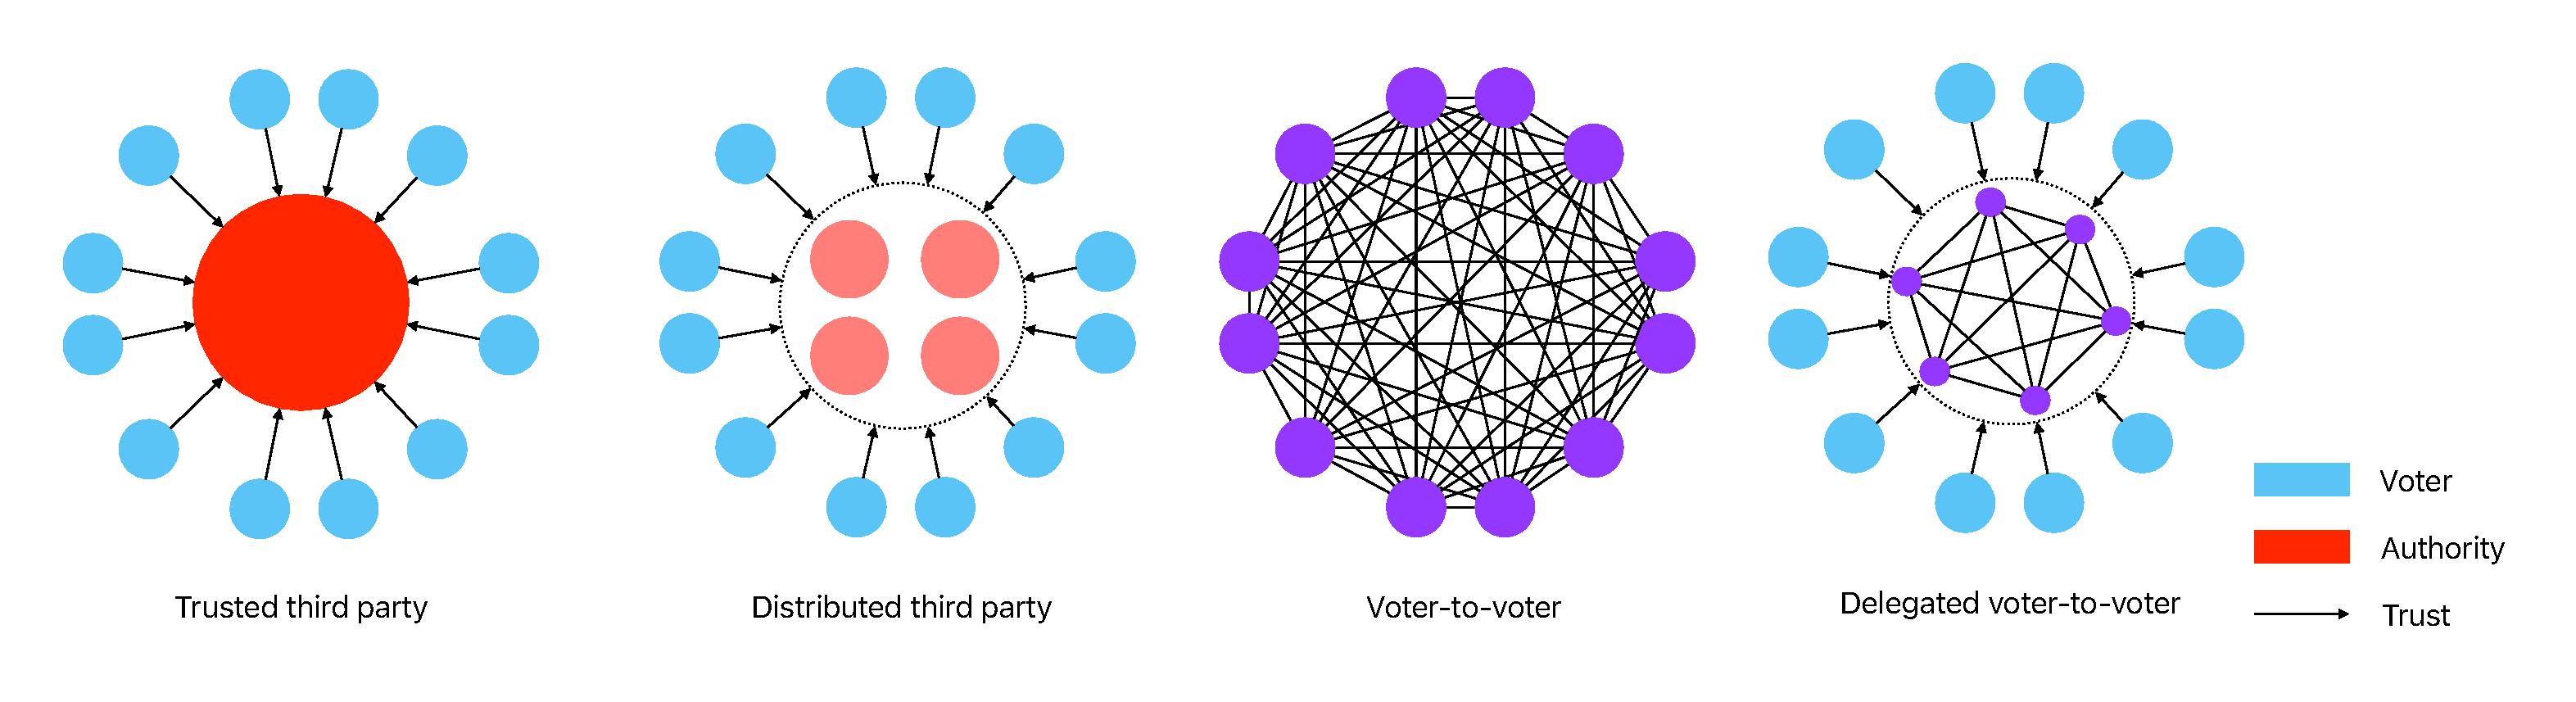
\includegraphics[width=\textwidth]{../paper/trust-models-voting.pdf}
\end{frame}

\begin{frame}
	\frametitle{Our Contributions}
	\begin{enumerate}
		\item Novel technique: Federated DKG (FDKG).
		\item Practicality with YOSO approach.
		\item Robustness through zkSNARKs.
		\item Privacy based on honest majority.
		\item Robust against faulty nodes.
		\item Cost-free for users.
	\end{enumerate}
\end{frame}

\begin{frame}
	\frametitle{Related Work: Trust in Internet Voting Protocols}
	\begin{itemize}
		\item Most rely on a trusted third party.
		\item Trust determines properties: anonymity, privacy, coercion resistance.
	\end{itemize}
\end{frame}

\begin{frame}
	\frametitle{Blockchain in Voting Protocols}
	\begin{itemize}
		\item Blockchain provides integral and transparent storage.
		\item Examples: Voatz, Polys, OpenVoteNetwork, MACI.
	\end{itemize}
\end{frame}


\begin{frame}
	\frametitle{Non-Blockchain Voting Protocols}
	\begin{itemize}
		\item Use distributed authorities for voting process (e.g., Civitas, Swisspost/Scytl, iVoting, ElectionGuard).
		\item Trust model: $N \textrm{ of } N$.
		\item Computation via Multi-Party Computation (MPC) protocol.
		\item Trusted entities called Guardians.
	\end{itemize}
\end{frame}

\begin{frame}
	\frametitle{Cost Implications in Voting Solutions}
	\begin{itemize}
		\item Public blockchains: Voters pay transaction fees.
		\item Private blockchains: Hosting costs or high entry for non-technical users.
		\item Voter-to-Voter network: No centralized server or transaction fees.
	\end{itemize}
\end{frame}

\begin{frame}
	\frametitle{Comparative Analysis}
	\begin{table}
	\centering
	\newcommand{\YES}{\cellcolor{red!50}Yes}
	\newcommand{\NO}{\cellcolor{green!50}No}
	\caption{Comparative analysis of internet voting systems.}
	\begin{tabular}{|l|l|l|l|l|}
	\hline
	\textbf{Property} & \textbf{Centralised} & \textbf{Private Infra.} & \textbf{Public Blockchain} & \textbf{Voter-to-Voter} \\
	\hline
	Transaction fees & \NO & \NO & \YES & \NO \\
	\hline
	Service costs & Medium & High & No  & No \\
	\hline
	User-Friendliness & High & High & Low & Medium \\
	\hline
	Trust to & Central authority & Authorities & Miners & Voters  \\
	\hline
	\end{tabular}
	\end{table}
\end{frame}

\begin{frame}
	\frametitle{Conclusion of Related Work}
	\begin{itemize}
		\item Trust remains a pivotal concern in internet voting protocols.
		\item Blockchain presents both opportunities and challenges.
		\item Need to weigh between cost, user-friendliness, and trust dynamics.
	\end{itemize}
\end{frame}

\begin{frame}{Internet voting is hard}
	Analysis of this area quickly reveals several unsolved issues.
	Secure voting requires four main properties

	\begin{itemize}
	\item<1-> \textbf{Correctness}, all and only eligible votes are counted.
	\item<2-> \textbf{Censorship resistance}, any eligible user that wants to cast a vote can do it.
	\item<3-> \textbf{Privacy}, no one can tell which candidate the voters voted for, or even if they voted at all—preventing preliminary results and guaranteeing freedom of choice.
	\item<4-> \textbf{Coercion resistance}, voters can not prove to anyone how they voted even if they want to—preventing selling votes as there is no way of verifying if they indeed voted on the paid candidate.
	\end{itemize}

	\pause
	They are hard to satisfy together
\end{frame}


\section{Internet votings}

\section{Contribution}

\section{Voter-to-Voter internet voting}

\section{Roadmap}

%%% PG LAST PAGE %%%
\pglastframe


%%% DOCUMENT ENDS HERE. Good bye! :) %%%

\end{document}

